\chapter{February Baseline: Dipole in Free Space versus Plasma}
\label{ch:february}

\section{What we tried}

After the January 2026 modernization (modular sources, CMake, OpenMP, Python plotting), the first physics question was whether the rebuilt solver could show plasma loading of a dipole at all. That is the prerequisite for later asking whether a vacuum sheath \emph{changes} that loading.

All February runs used the same antenna that later became \texttt{sheath.str}: \(70\times 70\times 65\) cells, \(\Delta x=\SI{0.04}{\meter}\), PEC from \((35,35,20)\) to \((35,35,45)\), feed at \((35,35,33)\), type-5 differentiated Gaussian. The only material difference from the May sheath input is the source parameter (\(\SI{100}{\mega\hertz}\) here versus \(\SI{30}{\kilo\hertz}\) later).

\begin{table}[ht]
\centering
\caption{February 2026 dipole runs under \texttt{results/}.}
\label{tab:feb-runs}
\begin{tabular}{@{}llll@{}}
\toprule
Run & Question & Settings & Outcome \\
\midrule
\texttt{production\_run\_8000} & Does OpenMP plasma run? & \(\fp=\SI{5.3}{\mega\hertz}\), \(f_c=\SI{1.43}{\mega\hertz}\), 8k steps & Yes: \(V/I\) and \(Z(f)\) plots \\
\texttt{freespace\_test} & Free-space dipole & no plasma CLI args, 100k steps & Baseline \(Z(f)\) \\
\texttt{ionoplasma\_test} & Plasma on, same dipole & \(\fp=\SI{0.5}{\mega\hertz}\), \(f_g=\SI{1.1}{\mega\hertz}\), 100k steps & Plasma-loaded \(Z(f)\) \\
\texttt{ionoplasma\_test\_5\_1\_11} & Collision / cyclotron variant & \(\fp=\SI{0.5}{\mega\hertz}\), \(f_c=\SI{0.05}{\mega\hertz}\), 64k steps & Parameter sensitivity \\
\texttt{benchmarks} & Legacy vs new OpenMP & \texttt{dipoleTest}, 10k steps & Timing, not physics \\
\texttt{test\_freespace} / \texttt{test\_plasma} & CLI plasma-flag check & \texttt{verify\_plasma\_flag.bat} & Incomplete (empty logs) \\
\bottomrule
\end{tabular}
\end{table}

\section{What succeeded}

The modernized OpenMP executable ran to completion. Free-space and plasma cases produced distinct voltage/current traces and impedance spectra (Figures~\ref{fig:feb-fs}--\ref{fig:feb-plasma}). The Python \(Z(f)=V(f)/I(f)\) pipeline used in every later chapter starts here. OpenMP scaling was recorded in Figure~\ref{fig:scaling}.

This established that \emph{plasma loading of feed impedance is measurable} on this grid. Without that result, a sheath-width sweep would have had no baseline.

\begin{figure}[ht]
\centering

\includegraphics[width=0.85\textwidth]{feb_freespace_impedance.png}
\caption{Free-space dipole impedance from \texttt{results/freespace\_test} (February 2026). Same geometry as all later sheath runs.}
\label{fig:feb-fs}
\end{figure}

\begin{figure}[ht]
\centering

\includegraphics[width=0.85\textwidth]{feb_ionoplasma_impedance.png}
\caption{Plasma-loaded dipole impedance from \texttt{results/ionoplasma\_test} (\(\fp=\SI{0.5}{\mega\hertz}\)). Plasma changes \(Z(f)\) relative to Figure~\ref{fig:feb-fs}.}
\label{fig:feb-plasma}
\end{figure}

\begin{figure}[ht]
\centering
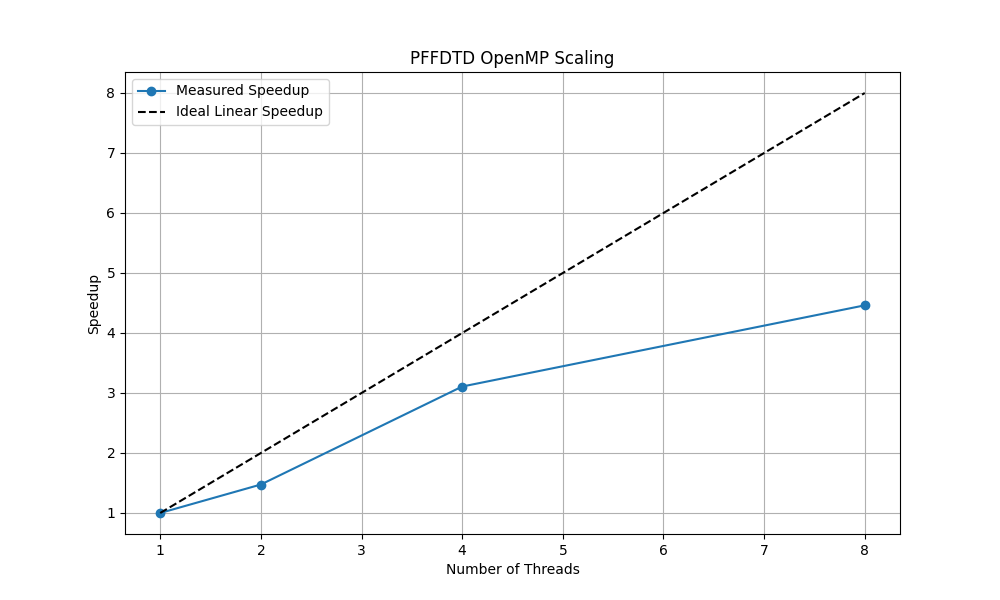
\includegraphics[width=0.75\textwidth]{scaling_results.png}
\caption{OpenMP scaling recorded during the February solver checkout.}
\label{fig:scaling}
\end{figure}

\section{What failed or was left open}

\begin{itemize}[leftmargin=1.5em]
\item There was no sheath parameter \(\Sd\). Density was spatially uniform.
\item Plasma frequencies (\(\SI{5.3}{\mega\hertz}\) or \(\SI{0.5}{\mega\hertz}\)) were Ward-like ionospheric defaults, not yet the Tu-oriented \(\SI{200}{\kilo\hertz}\) then \(\SI{2}{\mega\hertz}\) choices.
\item The \(\SI{100}{\mega\hertz}\) differentiated Gaussian is a broadband pulse. Frequency resolution and spectral artifacts from this class of drive reappear as a measurement failure in Chapter~\ref{ch:pulse}.
\item Several February runs included a cyclotron frequency (background \(\mathbf{B}\)). Later sheath work set \(f_{\mathrm{cyc}}=0\).
\item The CLI plasma-flag stubs (\texttt{test\_freespace}, \texttt{test\_plasma}) did not produce usable logs.
\end{itemize}

The May sheath campaign is the next chapter of this same antenna-in-plasma story: keep the dipole, add a vacuum layer of width \(\Sd\), and look for an upward shift of \(\fres\).
